\section{Phase 1: LPV representation validation}
\label{sec:phase1}

\subsection{Experiment 1A: frozen-grid matrix approximation}
\paragraph{Objective.}
Select the smallest LPV basis that accurately represents the discretized bicycle
models between measured speed anchors.

\paragraph{Predeclared expectation.}
The physically motivated reciprocal-speed basis is likely effective, but exact
discretization may make a richer mixed basis necessary.

\paragraph{Setup and planned evidence.}
For every client, calculate exact frozen discrete matrices and fit
\begin{align}
 \Phi_1(v)&=[1,v],\\
 \Phi_2(v)&=[1,v^{-1},v^{-2}],\\
 \Phi_3(v)&=[1,v,v^{-1},v^{-2}].
\end{align}
Fit on the five training anchors and evaluate at unseen intermediate speeds and a
dense grid. Report absolute and normalized $E_A(v)$ and $E_B(v)$, worst-client
error, coefficient magnitude, and regression conditioning.

\paragraph{Decision gate.}
Choose the smallest basis with consistently low interpolation error and acceptable
conditioning. The originally proposed basis is rejected if the evidence favors a
different representation.

\paragraph{Results, interpretation, and decision.}
The comparison was run on all 30 clients for each of the ten robustness seeds,
giving 300 independently perturbed vehicles.  Each model was fit to exact ZOH
matrices at $v=\{12,16,20,24,28\}\,\mathrm{m\,s^{-1}}$.  The unseen points
$v=\{14,18,22,26\}\,\mathrm{m\,s^{-1}}$ measure interpolation, while a
201-point grid over $[10,30]\,\mathrm{m\,s^{-1}}$ also tests the two edge
intervals outside the fitting anchors.  Nonconstant feature columns were
standardized before least squares.  Table~\ref{tab:experiment-1a} reports the
combined relative error
\begin{equation}
 e_{AB}=\sqrt{\frac{1}{2}\left(e_A^2+e_B^2\right)},\qquad
 e_A=\frac{\lVert\widehat A_d-A_d\rVert_F}{\lVert A_d\rVert_F},
\end{equation}
with $e_B$ defined analogously.

\begin{table}[htbp]
 \centering
 \caption{Experiment 1A basis comparison over 300 clients.  Error entries are
 percentages; ``full worst'' includes edge extrapolation to 10 and
 $30\,\mathrm{m\,s^{-1}}$.}
 \label{tab:experiment-1a}
 \begin{tabular}{lrrrrr}
  \toprule
  Basis & Terms & $\kappa_2$ & Interp. mean & Interp. worst & Full worst \\
  \midrule
  $[1,v]$ & 2 & 1.00 & $3.222\!\times\!10^{-1}$ & $6.607\!\times\!10^{-1}$ & 2.255 \\
  $[1,v^{-1},v^{-2}]$ & 3 & 17.51 & $6.814\!\times\!10^{-5}$ & $2.711\!\times\!10^{-4}$ & $2.266\!\times\!10^{-3}$ \\
  Mixed & 4 & 140.72 & $1.820\!\times\!10^{-5}$ & $7.137\!\times\!10^{-5}$ & $1.065\!\times\!10^{-3}$ \\
  \bottomrule
 \end{tabular}
\end{table}

\begin{figure}[htbp]
 \centering
 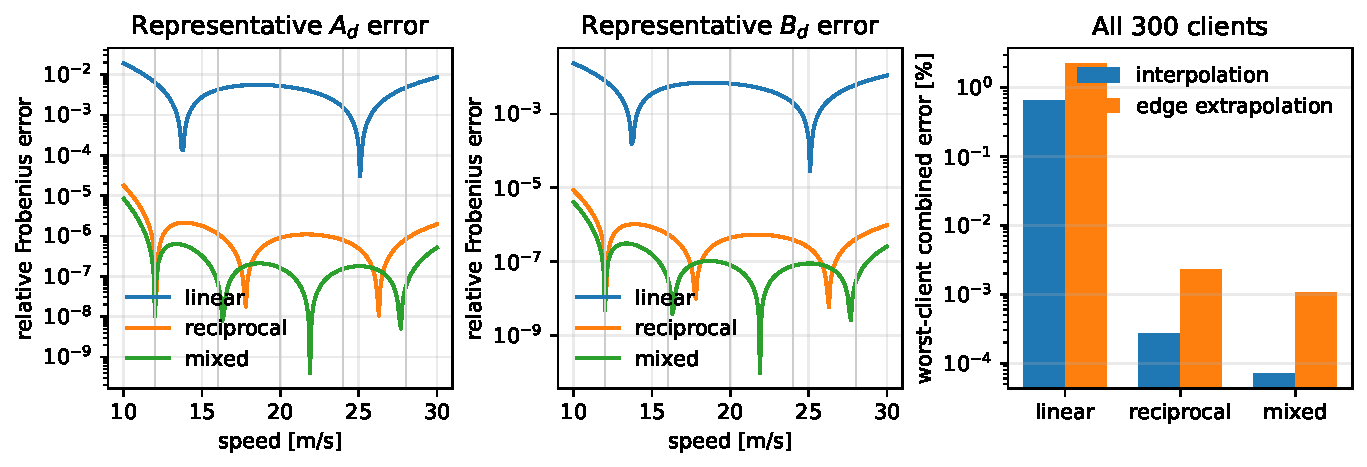
\includegraphics[width=\linewidth]{../results/figures/experiment_1a_basis_errors.pdf}
 \caption{Experiment 1A relative matrix errors.  The first two panels show a
 representative nominal client; gray lines mark fitting anchors.  The final
 panel gives population worst cases on a logarithmic scale.}
 \label{fig:experiment-1a}
\end{figure}

The error curves and population worst cases in \cref{fig:experiment-1a} confirm
the numerical ranking in \cref{tab:experiment-1a} over the full speed envelope.

The linear basis reaches a 2.26\% worst-case full-envelope error, which is too
large compared with the method differences that later experiments seek to
resolve.  The reciprocal basis reduces this error by roughly three orders of
magnitude to 0.00227\%.  Adding the $v$ term halves an already negligible error,
but increases the standardized design-matrix condition number from 17.5 to
140.7 and adds another coefficient matrix.  The largest reciprocal-basis error
occurs in edge extrapolation; its worst unseen-interpolation error is only
$2.71\times10^{-4}$\%.

Experiment 1A therefore passes.  We select and provisionally freeze
\begin{equation}
 \boxed{\Phi(v)=[1,v^{-1},v^{-2}]}
\end{equation}
as the smallest sufficiently accurate representation.  Experiment 1B must now
verify that this pointwise result remains accurate under time-varying simulation.

\subsection{Experiment 1B: varying-speed trajectory prediction}
\paragraph{Objective.}
Confirm that pointwise matrix accuracy translates into accurate speed-varying
simulation.

\paragraph{Predeclared expectation.}
The chosen LPV basis gives nearly exact one-step prediction and small, bounded
free-run error on the linear plant.

\paragraph{Setup and planned evidence.}
Use moderate persistently exciting steering with independent smooth profiles such
as $12\rightarrow20\rightarrow15$, $20\rightarrow28\rightarrow18$, and
$15\rightarrow25\rightarrow12\,\mathrm{m\,s^{-1}}$. Compare the true
speed-varying plant, exact frozen-matrix lookup, and fitted LPV model. Plot
representative states and error versus time, speed, and client family.

\paragraph{Decision gate.}
One-step errors must be negligible relative to the later between-method effects,
and free-run errors must not grow pathologically. Otherwise the basis or the
time-varying discretization treatment is revised before Phase~2.

\paragraph{Results, interpretation, and decision.}
The experiment used three smooth speed profiles,
$12\rightarrow20\rightarrow15$, $20\rightarrow28\rightarrow18$, and
$15\rightarrow25\rightarrow12\,\mathrm{m\,s^{-1}}$, each lasting 12 seconds.
All profiles were paired with the same independent three-frequency multisine
steering signal, whose peak magnitude is below $2.2^\circ$.  This common input
prevents speed and maneuver differences from being confounded.  The evaluation
again covered all 300 vehicles from the ten robustness seeds, for 900
trajectories in total.

The reference trajectory was integrated by fourth-order Runge--Kutta while
evaluating $A(v(t))$ and $B(v(t))$ continuously inside each sample.  Two
scheduled discrete models were propagated recursively: exact ZOH matrices
frozen at the left sample speed and the fitted reciprocal LPV matrices.  A third
comparison evaluates the LPV trajectory directly against the exact scheduled
discrete trajectory, thereby isolating basis approximation from the shared
sample-wise freezing error.  Relative errors are normalized by the RMS norm of
the corresponding reference state trajectory.

\begin{table}[htbp]
 \centering
 \caption{Experiment 1B one-step and free-run relative RMSE over 900
 trajectories. All error entries are percentages.}
 \label{tab:experiment-1b}
 \begin{tabular}{lrrrr}
  \toprule
  Comparison & 1-step avg. & 1-step max. & Free avg. & Free max. \\
  \midrule
  Exact frozen vs. continuous & $2.102\!\times\!10^{-3}$ & $3.275\!\times\!10^{-3}$ & $2.139\!\times\!10^{-2}$ & $3.339\!\times\!10^{-2}$ \\
  Reciprocal LPV vs. continuous & $2.116\!\times\!10^{-3}$ & $3.297\!\times\!10^{-3}$ & $2.184\!\times\!10^{-2}$ & $3.358\!\times\!10^{-2}$ \\
  Reciprocal LPV vs. exact frozen & $8.532\!\times\!10^{-5}$ & $1.725\!\times\!10^{-4}$ & $2.461\!\times\!10^{-3}$ & $6.112\!\times\!10^{-3}$ \\
  \bottomrule
 \end{tabular}
\end{table}

\begin{figure}[htbp]
 \centering
 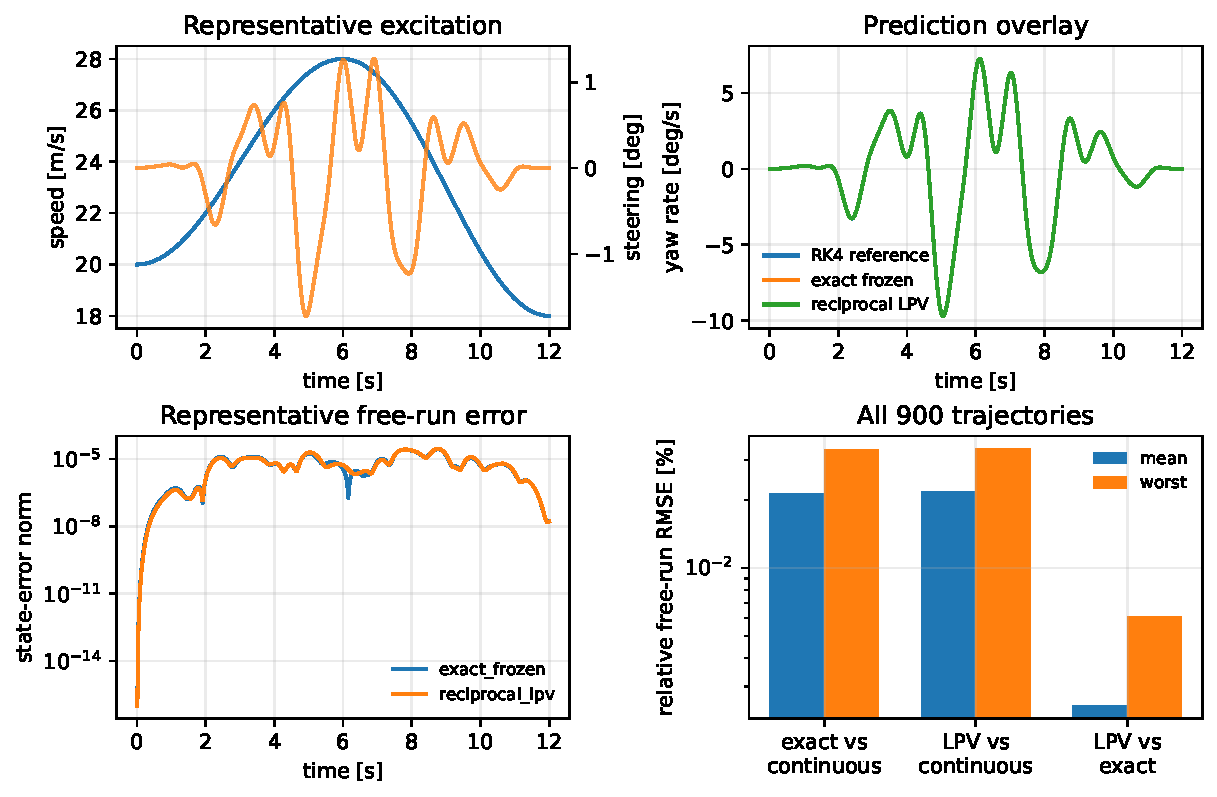
\includegraphics[width=0.92\linewidth]{../results/figures/experiment_1b_trajectory_validation.pdf}
 \caption{Experiment 1B varying-speed validation.  The scheduled predictions
 overlap visually with the continuous-time reference.  The lower panels expose
 the small free-run errors and distinguish the LPV basis error from the common
 within-sample speed-freezing error.}
 \label{fig:experiment-1b}
\end{figure}

The representative trajectories and separated error components are shown in
\cref{fig:experiment-1b}; the aggregate errors are reported in
\cref{tab:experiment-1b}.

The fitted LPV model is visually indistinguishable from both references.  Its
worst free-run error against the continuous-speed plant is only 0.0336\%, with
worst physical RMSEs of $4.78\times10^{-4}$ degrees in sideslip and
$1.15\times10^{-3}\,\mathrm{deg\,s^{-1}}$ in yaw rate.  Most of this discrepancy
is already present for exact frozen matrices.  The isolated reciprocal-basis
contribution has 0.00246\% mean and 0.00611\% worst free-run RMSE.  Its worst
one-step error is $1.73\times10^{-4}$\%.  Errors remain bounded throughout each
maneuver and decay with the faded input, rather than accumulating
pathologically.

Experiment 1B therefore passes.  The reciprocal representation is sufficiently
accurate that its approximation error is negligible relative to the effects
targeted in the oracle architecture comparison.

\subsection{Phase-1 representation freeze}
Experiments 1A and 1B jointly validate and freeze the Phase-1 representation:
\begin{itemize}
 \item scheduling basis $\Phi(v)=[1,v^{-1},v^{-2}]$;
 \item standardized nonconstant regression features;
 \item exact ZOH target matrices at $T_s=0.01\,\mathrm{s}$;
 \item fitting anchors $v=\{12,16,20,24,28\}\,\mathrm{m\,s^{-1}}$.
\end{itemize}
These choices remain fixed in the Phase-2 oracle comparison.  The validated
model is still the linear-tire bicycle plant; the nonlinear tanh-tire benchmark
remains a later robustness layer after the core architectural claim is tested.
